%%%% Figure Comparison: More variants
\documentclass{article}
\pdfpagewidth=8.5in
\pdfpageheight=11in

\usepackage{ijcai26}
\usepackage{times}
\usepackage[hidelinks]{hyperref}
\usepackage[utf8]{inputenc}
\usepackage[small]{caption}
\usepackage{graphicx}
\usepackage{tikz}
\usepackage{xcolor}

\usetikzlibrary{shapes.geometric, arrows.meta, positioning, fit, backgrounds, calc, decorations.pathmorphing, patterns}

\definecolor{clrPrompt}{HTML}{B0CA97}
\definecolor{clrBatch}{HTML}{88C4C8}
\definecolor{clrEval}{HTML}{D1BC8A}
\definecolor{clrOutcome}{HTML}{E8A087}
\definecolor{clrExpert}{HTML}{D1BC8A}
\definecolor{clrDev}{HTML}{88C4C8}
\definecolor{clrExpertK}{HTML}{C9B3D9}   % lavender — distinct from blue & beige
\definecolor{clrDevK}{HTML}{F0C0C0}      % blush pink — distinct from blue & beige

\title{LLARS Figure Variants}
\author{}

\begin{document}
\maketitle


%% ============================================================
%% VARIANT E3b: E3 polished — colored boxes, dotted separator
%% ============================================================

\begin{figure*}[t]
\centering
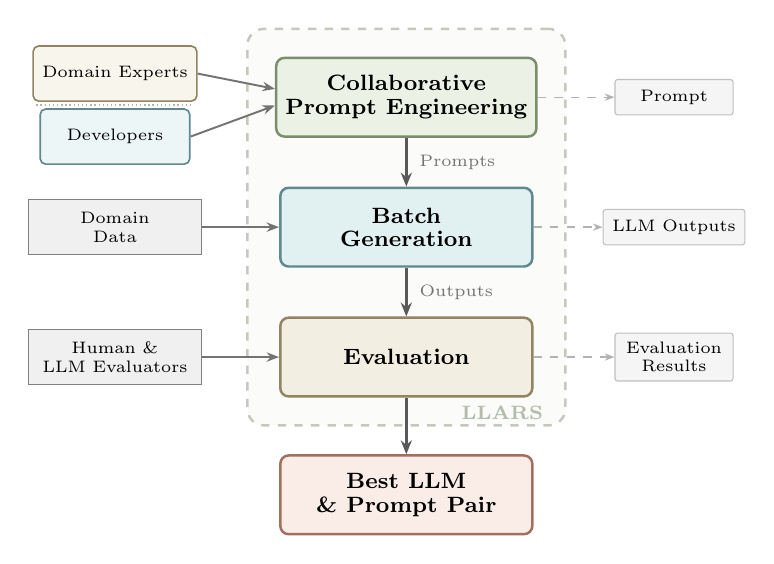
\begin{tikzpicture}[
    module/.style={rectangle, minimum width=3.2cm, minimum height=1.0cm, align=center, font=\footnotesize\bfseries, rounded corners=3pt, line width=0.9pt},
    actor/.style={rectangle, draw=black!50, fill=black!6, minimum width=2.2cm, minimum height=0.7cm, align=center, font=\fontsize{6.5}{8}\selectfont, line width=0.5pt},
    actorrole/.style={rectangle, minimum width=1.9cm, minimum height=0.7cm, align=center, font=\fontsize{6.5}{8}\selectfont, line width=0.6pt},
    export/.style={rectangle, draw=black!25, fill=black!4, minimum width=1.5cm, minimum height=0.45cm, align=center, font=\fontsize{6}{7.5}\selectfont, rounded corners=1pt},
    outcome/.style={rectangle, draw=clrOutcome!70!black, fill=clrOutcome!20, minimum width=3.2cm, minimum height=1.0cm, align=center, font=\footnotesize\bfseries, rounded corners=3pt, line width=0.9pt},
    arrow/.style={-{Stealth[length=4.5pt]}, line width=0.7pt, black!55},
    pipearrow/.style={-{Stealth[length=5pt, width=4pt]}, line width=1.0pt, black!65},
    dasharrow/.style={-{Stealth[length=3.5pt]}, line width=0.5pt, black!30, dashed},
    lbl/.style={font=\fontsize{6}{7.5}\selectfont, text=black!55},
]

\node[module, draw=clrPrompt!70!black, fill=clrPrompt!25] (pe) at (0, 0) {Collaborative\\[-1pt]Prompt Engineering};
\node[module, draw=clrBatch!70!black, fill=clrBatch!25] (bg) at (0, -1.65) {Batch\\[-1pt]Generation};
\node[module, draw=clrEval!70!black, fill=clrEval!25] (ev) at (0, -3.3) {Evaluation};

% Split actor boxes with color coding
\node[actorrole, draw=clrExpert!70!black, fill=clrExpert!15, rounded corners=2pt] (experts) at (-3.7, 0.3) {Domain Experts};
\node[actorrole, draw=clrDev!70!black, fill=clrDev!15, rounded corners=2pt] (devs) at (-3.7, -0.5) {Developers};

% Dotted line separator
\draw[black!30, line width=0.5pt, densely dotted] (-4.7, -0.1) -- (-2.7, -0.1);

\draw[arrow] (experts.east) -- ([yshift=3pt]pe.west);
\draw[arrow] (devs.east) -- ([yshift=-3pt]pe.west);

\node[actor] (data) at (-3.7, -1.65) {Domain\\[-1pt]Data};
\node[actor] (llmeval) at (-3.7, -3.3) {Human \&\\[-1pt]LLM Evaluators};
\draw[arrow] (data.east) -- (bg.west);
\draw[arrow] (llmeval.east) -- (ev.west);

\draw[pipearrow] (pe.south) -- node[lbl, right, xshift=1pt] {Prompts} (bg.north);
\draw[pipearrow] (bg.south) -- node[lbl, right, xshift=1pt] {Outputs} (ev.north);

\node[export] (exp1) at (3.4, 0) {Prompt};
\node[export] (exp2) at (3.4, -1.65) {LLM Outputs};
\node[export] (exp3) at (3.4, -3.3) {Evaluation\\[-1pt]Results};
\draw[dasharrow] (pe.east) -- (exp1);
\draw[dasharrow] (bg.east) -- (exp2);
\draw[dasharrow] (ev.east) -- (exp3);

\node[outcome] (outcome) at (0, -5.05) {Best LLM \\[-1pt]\& Prompt Pair};
\draw[pipearrow] (ev.south) -- (outcome.north);

\begin{scope}[on background layer]
\node[draw=clrPrompt!60!black!40, dashed, rounded corners=6pt, line width=0.9pt, fill=clrPrompt!5, fit=(pe)(bg)(ev), inner xsep=10pt, inner ysep=10pt] (llarsbox) {};
\node[font=\fontsize{7}{9}\selectfont\bfseries, text=clrPrompt!60!black!50, anchor=south east] at ([xshift=-5pt, yshift=-1pt]llarsbox.south east) {LLARS};
\end{scope}

\end{tikzpicture}
\caption{\textbf{E3b:} E3 polished with color-coded role boxes (warm = experts, cool = developers) and a dotted separator. Minimal change to original.}
\end{figure*}


%% ============================================================
%% VARIANT F: Bridge arc connecting two sides
%% ============================================================

\begin{figure*}[t]
\centering
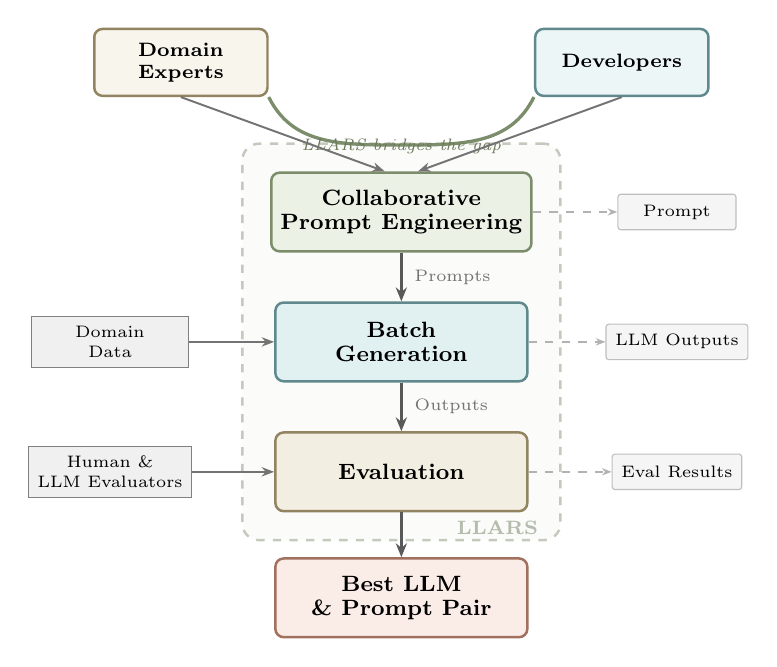
\begin{tikzpicture}[
    module/.style={rectangle, minimum width=3.2cm, minimum height=1.0cm, align=center, font=\footnotesize\bfseries, rounded corners=3pt, line width=0.9pt},
    actorrole/.style={rectangle, minimum width=2.2cm, minimum height=0.85cm, align=center, font=\fontsize{7}{9}\selectfont\bfseries, rounded corners=3pt, line width=0.9pt},
    actor/.style={rectangle, draw=black!50, fill=black!6, minimum width=2.0cm, minimum height=0.65cm, align=center, font=\fontsize{6.5}{8}\selectfont, line width=0.5pt},
    export/.style={rectangle, draw=black!25, fill=black!4, minimum width=1.5cm, minimum height=0.45cm, align=center, font=\fontsize{6}{7.5}\selectfont, rounded corners=1pt},
    outcome/.style={rectangle, draw=clrOutcome!70!black, fill=clrOutcome!20, minimum width=3.2cm, minimum height=1.0cm, align=center, font=\footnotesize\bfseries, rounded corners=3pt, line width=0.9pt},
    arrow/.style={-{Stealth[length=4.5pt]}, line width=0.7pt, black!55},
    pipearrow/.style={-{Stealth[length=5pt, width=4pt]}, line width=1.0pt, black!65},
    dasharrow/.style={-{Stealth[length=3.5pt]}, line width=0.5pt, black!30, dashed},
    lbl/.style={font=\fontsize{6}{7.5}\selectfont, text=black!55},
]

% Top: Two groups
\node[actorrole, draw=clrExpert!70!black, fill=clrExpert!15] (experts) at (-2.8, 1.0) {Domain\\[-1pt]Experts};
\node[actorrole, draw=clrDev!70!black, fill=clrDev!15] (devs) at (2.8, 1.0) {Developers};

% Bridge arc
\draw[clrPrompt!70!black, line width=1.2pt]
    (experts.south east) .. controls ($(experts.south east)+(0.3,-0.6)$) and ($(-0.8, -0.05)$) .. (0, -0.05)
    .. controls ($(0.8, -0.05)$) and ($(devs.south west)+(-0.3,-0.6)$) .. (devs.south west);

% Bridge label
\node[font=\fontsize{6}{7.5}\selectfont\itshape, text=clrPrompt!60!black, anchor=north] at (0, 0.15) {LLARS bridges the gap};

% Modules
\node[module, draw=clrPrompt!70!black, fill=clrPrompt!25] (pe) at (0, -0.9) {Collaborative\\[-1pt]Prompt Engineering};
\node[module, draw=clrBatch!70!black, fill=clrBatch!25] (bg) at (0, -2.55) {Batch\\[-1pt]Generation};
\node[module, draw=clrEval!70!black, fill=clrEval!25] (ev) at (0, -4.2) {Evaluation};

% Arrows from actors into pipeline
\draw[arrow] (experts.south) -- ([xshift=-6pt]pe.north);
\draw[arrow] (devs.south) -- ([xshift=6pt]pe.north);

% Side actors
\node[actor] (data) at (-3.7, -2.55) {Domain\\[-1pt]Data};
\node[actor] (heval) at (-3.7, -4.2) {Human \&\\[-1pt]LLM Evaluators};
\draw[arrow] (data.east) -- (bg.west);
\draw[arrow] (heval.east) -- (ev.west);

% Pipeline
\draw[pipearrow] (pe.south) -- node[lbl, right, xshift=1pt] {Prompts} (bg.north);
\draw[pipearrow] (bg.south) -- node[lbl, right, xshift=1pt] {Outputs} (ev.north);

% Export
\node[export] (exp1) at (3.5, -0.9) {Prompt};
\node[export] (exp2) at (3.5, -2.55) {LLM Outputs};
\node[export] (exp3) at (3.5, -4.2) {Eval Results};
\draw[dasharrow] (pe.east) -- (exp1);
\draw[dasharrow] (bg.east) -- (exp2);
\draw[dasharrow] (ev.east) -- (exp3);

% Outcome
\node[outcome] (outcome) at (0, -5.8) {Best LLM \\[-1pt]\& Prompt Pair};
\draw[pipearrow] (ev.south) -- (outcome.north);

\begin{scope}[on background layer]
\node[draw=clrPrompt!60!black!40, dashed, rounded corners=6pt, line width=0.9pt, fill=clrPrompt!5, fit=(pe)(bg)(ev), inner xsep=10pt, inner ysep=10pt] (llarsbox) {};
\node[font=\fontsize{7}{9}\selectfont\bfseries, text=clrPrompt!60!black!50, anchor=south east] at ([xshift=-5pt, yshift=-1pt]llarsbox.south east) {LLARS};
\end{scope}

\end{tikzpicture}
\caption{\textbf{F:} Bridge arc connecting Domain Experts and Developers over the pipeline. Explicit ``bridges the gap'' label.}
\end{figure*}


%% ============================================================
%% VARIANT G: Role participation bars per module
%% ============================================================

\begin{figure*}[t]
\centering
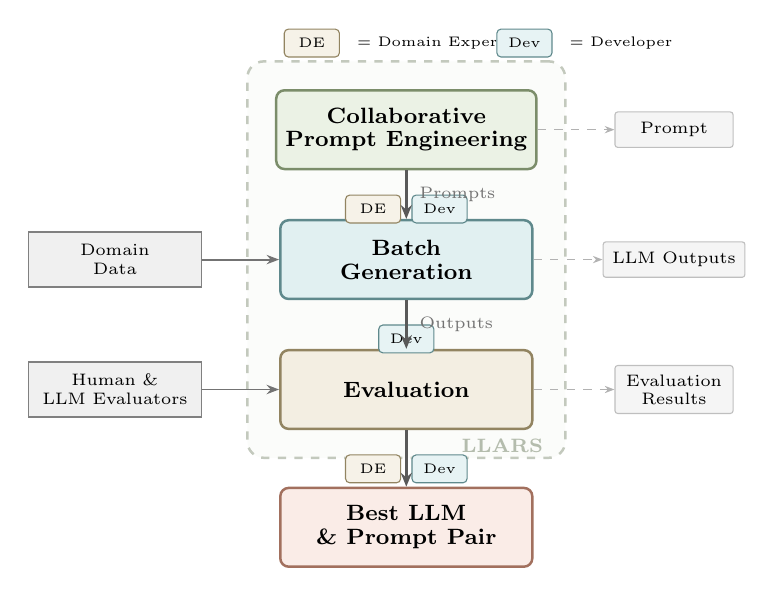
\begin{tikzpicture}[
    module/.style={rectangle, minimum width=3.2cm, minimum height=1.0cm, align=center, font=\footnotesize\bfseries, rounded corners=3pt, line width=0.9pt},
    actor/.style={rectangle, draw=black!50, fill=black!6, minimum width=2.2cm, minimum height=0.7cm, align=center, font=\fontsize{6.5}{8}\selectfont, line width=0.5pt},
    roletag/.style={rectangle, minimum width=0.7cm, minimum height=0.28cm, align=center, font=\fontsize{4.5}{5.5}\selectfont, rounded corners=1.5pt, line width=0.4pt},
    export/.style={rectangle, draw=black!25, fill=black!4, minimum width=1.5cm, minimum height=0.45cm, align=center, font=\fontsize{6}{7.5}\selectfont, rounded corners=1pt},
    outcome/.style={rectangle, draw=clrOutcome!70!black, fill=clrOutcome!20, minimum width=3.2cm, minimum height=1.0cm, align=center, font=\footnotesize\bfseries, rounded corners=3pt, line width=0.9pt},
    arrow/.style={-{Stealth[length=4.5pt]}, line width=0.7pt, black!55},
    pipearrow/.style={-{Stealth[length=5pt, width=4pt]}, line width=1.0pt, black!65},
    dasharrow/.style={-{Stealth[length=3.5pt]}, line width=0.5pt, black!30, dashed},
    lbl/.style={font=\fontsize{6}{7.5}\selectfont, text=black!55},
]

% Legend at top
\node[roletag, draw=clrExpert!70!black, fill=clrExpert!20] (leg1) at (-1.2, 1.1) {DE};
\node[font=\fontsize{5.5}{7}\selectfont, anchor=west] at (-0.75, 1.1) {= Domain Expert};
\node[roletag, draw=clrDev!70!black, fill=clrDev!20] (leg2) at (1.5, 1.1) {Dev};
\node[font=\fontsize{5.5}{7}\selectfont, anchor=west] at (1.95, 1.1) {= Developer};

% Modules
\node[module, draw=clrPrompt!70!black, fill=clrPrompt!25] (pe) at (0, 0) {Collaborative\\[-1pt]Prompt Engineering};
\node[module, draw=clrBatch!70!black, fill=clrBatch!25] (bg) at (0, -1.65) {Batch\\[-1pt]Generation};
\node[module, draw=clrEval!70!black, fill=clrEval!25] (ev) at (0, -3.3) {Evaluation};

% Role tags on modules (who participates where)
% Prompt Engineering: both
\node[roletag, draw=clrExpert!70!black, fill=clrExpert!20] at ([xshift=-12pt, yshift=-14pt]pe.south) {DE};
\node[roletag, draw=clrDev!70!black, fill=clrDev!20] at ([xshift=12pt, yshift=-14pt]pe.south) {Dev};
% Batch Generation: mainly developer
\node[roletag, draw=clrDev!70!black, fill=clrDev!20] at ([xshift=0pt, yshift=-14pt]bg.south) {Dev};
% Evaluation: both + LLM
\node[roletag, draw=clrExpert!70!black, fill=clrExpert!20] at ([xshift=-12pt, yshift=-14pt]ev.south) {DE};
\node[roletag, draw=clrDev!70!black, fill=clrDev!20] at ([xshift=12pt, yshift=-14pt]ev.south) {Dev};

% Left actors
\node[actor] (data) at (-3.7, -1.65) {Domain\\[-1pt]Data};
\node[actor] (llmeval) at (-3.7, -3.3) {Human \&\\[-1pt]LLM Evaluators};
\draw[arrow] (data.east) -- (bg.west);
\draw[arrow] (llmeval.east) -- (ev.west);

% Pipeline
\draw[pipearrow] (pe.south) -- node[lbl, right, xshift=1pt] {Prompts} (bg.north);
\draw[pipearrow] (bg.south) -- node[lbl, right, xshift=1pt] {Outputs} (ev.north);

% Export
\node[export] (exp1) at (3.4, 0) {Prompt};
\node[export] (exp2) at (3.4, -1.65) {LLM Outputs};
\node[export] (exp3) at (3.4, -3.3) {Evaluation\\[-1pt]Results};
\draw[dasharrow] (pe.east) -- (exp1);
\draw[dasharrow] (bg.east) -- (exp2);
\draw[dasharrow] (ev.east) -- (exp3);

% Outcome
\node[outcome] (outcome) at (0, -5.05) {Best LLM \\[-1pt]\& Prompt Pair};
\draw[pipearrow] (ev.south) -- (outcome.north);

\begin{scope}[on background layer]
\node[draw=clrPrompt!60!black!40, dashed, rounded corners=6pt, line width=0.9pt, fill=clrPrompt!5, fit=(pe)(bg)(ev), inner xsep=10pt, inner ysep=10pt] (llarsbox) {};
\node[font=\fontsize{7}{9}\selectfont\bfseries, text=clrPrompt!60!black!50, anchor=south east] at ([xshift=-5pt, yshift=-1pt]llarsbox.south east) {LLARS};
\end{scope}

\end{tikzpicture}
\caption{\textbf{G:} Role participation tags on each module show which roles work where. Domain Experts and Developers both appear in Prompt Engineering and Evaluation; Developers drive Batch Generation.}
\end{figure*}


%% ============================================================
%% VARIANT H: Horizontal top bar — two roles, one shared platform
%% ============================================================

\begin{figure*}[t]
\centering
\begin{tikzpicture}[
    module/.style={rectangle, minimum width=3.2cm, minimum height=1.0cm, align=center, font=\footnotesize\bfseries, rounded corners=3pt, line width=0.9pt},
    actor/.style={rectangle, draw=black!50, fill=black!6, minimum width=2.0cm, minimum height=0.65cm, align=center, font=\fontsize{6.5}{8}\selectfont, line width=0.5pt},
    export/.style={rectangle, draw=black!25, fill=black!4, minimum width=1.5cm, minimum height=0.45cm, align=center, font=\fontsize{6}{7.5}\selectfont, rounded corners=1pt},
    outcome/.style={rectangle, draw=clrOutcome!70!black, fill=clrOutcome!20, minimum width=3.2cm, minimum height=1.0cm, align=center, font=\footnotesize\bfseries, rounded corners=3pt, line width=0.9pt},
    arrow/.style={-{Stealth[length=4.5pt]}, line width=0.7pt, black!55},
    pipearrow/.style={-{Stealth[length=5pt, width=4pt]}, line width=1.0pt, black!65},
    dasharrow/.style={-{Stealth[length=3.5pt]}, line width=0.5pt, black!30, dashed},
    lbl/.style={font=\fontsize{6}{7.5}\selectfont, text=black!55},
]

% === Horizontal top bar: two role boxes side by side ===
\node[rectangle, draw=clrExpert!70!black, fill=clrExpert!15, minimum width=2.4cm, minimum height=0.7cm, align=center, font=\fontsize{6.5}{8}\selectfont\bfseries, rounded corners=2pt, line width=0.6pt] (experts) at (-1.4, 0.9) {Domain Experts};
\node[rectangle, draw=clrDev!70!black, fill=clrDev!15, minimum width=2.4cm, minimum height=0.7cm, align=center, font=\fontsize{6.5}{8}\selectfont\bfseries, rounded corners=2pt, line width=0.6pt] (devs) at (1.4, 0.9) {Developers};

% Thin connecting line underneath (shared platform)
\draw[clrPrompt!60!black, line width=1.0pt] (-2.7, 0.45) -- (2.7, 0.45);
\node[font=\fontsize{5}{6.5}\selectfont\itshape, text=clrPrompt!60!black, anchor=north] at (0, 0.42) {shared platform};

% Arrows down into first module
\draw[arrow] (0, 0.35) -- (pe.north);

% Modules
\node[module, draw=clrPrompt!70!black, fill=clrPrompt!25] (pe) at (0, -0.5) {Collaborative\\[-1pt]Prompt Engineering};
\node[module, draw=clrBatch!70!black, fill=clrBatch!25] (bg) at (0, -2.15) {Batch\\[-1pt]Generation};
\node[module, draw=clrEval!70!black, fill=clrEval!25] (ev) at (0, -3.8) {Evaluation};

% Left actors
\node[actor] (data) at (-3.7, -2.15) {Domain\\[-1pt]Data};
\node[actor] (llmeval) at (-3.7, -3.8) {Human \&\\[-1pt]LLM Evaluators};
\draw[arrow] (data.east) -- (bg.west);
\draw[arrow] (llmeval.east) -- (ev.west);

% Pipeline
\draw[pipearrow] (pe.south) -- node[lbl, right, xshift=1pt] {Prompts} (bg.north);
\draw[pipearrow] (bg.south) -- node[lbl, right, xshift=1pt] {Outputs} (ev.north);

% Export
\node[export] (exp1) at (3.4, -0.5) {Prompt};
\node[export] (exp2) at (3.4, -2.15) {LLM Outputs};
\node[export] (exp3) at (3.4, -3.8) {Evaluation\\[-1pt]Results};
\draw[dasharrow] (pe.east) -- (exp1);
\draw[dasharrow] (bg.east) -- (exp2);
\draw[dasharrow] (ev.east) -- (exp3);

% Outcome
\node[outcome] (outcome) at (0, -5.55) {Best LLM \\[-1pt]\& Prompt Pair};
\draw[pipearrow] (ev.south) -- (outcome.north);

\begin{scope}[on background layer]
\node[draw=clrPrompt!60!black!40, dashed, rounded corners=6pt, line width=0.9pt, fill=clrPrompt!5, fit=(pe)(bg)(ev), inner xsep=10pt, inner ysep=10pt] (llarsbox) {};
\node[font=\fontsize{7}{9}\selectfont\bfseries, text=clrPrompt!60!black!50, anchor=south east] at ([xshift=-5pt, yshift=-1pt]llarsbox.south east) {LLARS};
\end{scope}

\end{tikzpicture}
\caption{\textbf{H:} Two role boxes at the top connected by a ``shared platform'' bar. Clean and understated — shows two groups entering the same system.}
\end{figure*}


%% ============================================================
%% VARIANT I: Two silos → shared LLARS (before/after feel)
%% ============================================================

\begin{figure*}[t]
\centering
\begin{tikzpicture}[
    module/.style={rectangle, minimum width=3.2cm, minimum height=1.0cm, align=center, font=\footnotesize\bfseries, rounded corners=3pt, line width=0.9pt},
    actor/.style={rectangle, draw=black!50, fill=black!6, minimum width=2.0cm, minimum height=0.65cm, align=center, font=\fontsize{6.5}{8}\selectfont, line width=0.5pt},
    export/.style={rectangle, draw=black!25, fill=black!4, minimum width=1.5cm, minimum height=0.45cm, align=center, font=\fontsize{6}{7.5}\selectfont, rounded corners=1pt},
    outcome/.style={rectangle, draw=clrOutcome!70!black, fill=clrOutcome!20, minimum width=3.2cm, minimum height=1.0cm, align=center, font=\footnotesize\bfseries, rounded corners=3pt, line width=0.9pt},
    arrow/.style={-{Stealth[length=4.5pt]}, line width=0.7pt, black!55},
    pipearrow/.style={-{Stealth[length=5pt, width=4pt]}, line width=1.0pt, black!65},
    dasharrow/.style={-{Stealth[length=3.5pt]}, line width=0.5pt, black!30, dashed},
    lbl/.style={font=\fontsize{6}{7.5}\selectfont, text=black!55},
    silo/.style={rectangle, minimum width=1.6cm, minimum height=0.5cm, align=center, font=\fontsize{5.5}{7}\selectfont, line width=0.5pt, rounded corners=1.5pt},
]

% === Top: Two isolated silo stacks ===
\node[silo, draw=clrExpert!70!black, fill=clrExpert!12] (e1) at (-2.3, 1.5) {Quality criteria};
\node[silo, draw=clrExpert!70!black, fill=clrExpert!12] (e2) at (-2.3, 0.85) {Domain feedback};
\node[rectangle, draw=clrExpert!70!black, fill=clrExpert!25, minimum width=1.8cm, minimum height=0.55cm, align=center, font=\fontsize{6}{7.5}\selectfont\bfseries, rounded corners=2pt, line width=0.6pt] (elbl) at (-2.3, 2.15) {Domain Experts};

\node[silo, draw=clrDev!70!black, fill=clrDev!12] (d1) at (2.3, 1.5) {Prompt design};
\node[silo, draw=clrDev!70!black, fill=clrDev!12] (d2) at (2.3, 0.85) {Model config};
\node[rectangle, draw=clrDev!70!black, fill=clrDev!25, minimum width=1.8cm, minimum height=0.55cm, align=center, font=\fontsize{6}{7.5}\selectfont\bfseries, rounded corners=2pt, line width=0.6pt] (dlbl) at (2.3, 2.15) {Developers};

% Gap between silos
\node[font=\fontsize{7}{9}\selectfont, text=black!30] at (0, 1.35) {\textbf{$\times$}};
\node[font=\fontsize{5}{6}\selectfont\itshape, text=black!30] at (0, 0.85) {isolated};

% Converging arrows
\draw[arrow, line width=0.8pt] (-2.3, 0.5) .. controls (-2.3, -0.1) and (-0.5, -0.3) .. ([xshift=-4pt]pe.north);
\draw[arrow, line width=0.8pt] (2.3, 0.5) .. controls (2.3, -0.1) and (0.5, -0.3) .. ([xshift=4pt]pe.north);

% Modules
\node[module, draw=clrPrompt!70!black, fill=clrPrompt!25] (pe) at (0, -0.9) {Collaborative\\[-1pt]Prompt Engineering};
\node[module, draw=clrBatch!70!black, fill=clrBatch!25] (bg) at (0, -2.55) {Batch\\[-1pt]Generation};
\node[module, draw=clrEval!70!black, fill=clrEval!25] (ev) at (0, -4.2) {Evaluation};

% Side actors
\node[actor] (data) at (-3.7, -2.55) {Domain\\[-1pt]Data};
\node[actor] (heval) at (-3.7, -4.2) {Human \&\\[-1pt]LLM Evaluators};
\draw[arrow] (data.east) -- (bg.west);
\draw[arrow] (heval.east) -- (ev.west);

% Pipeline
\draw[pipearrow] (pe.south) -- node[lbl, right, xshift=1pt] {Prompts} (bg.north);
\draw[pipearrow] (bg.south) -- node[lbl, right, xshift=1pt] {Outputs} (ev.north);

% Export
\node[export] (exp1) at (3.5, -0.9) {Prompt};
\node[export] (exp2) at (3.5, -2.55) {LLM Outputs};
\node[export] (exp3) at (3.5, -4.2) {Eval Results};
\draw[dasharrow] (pe.east) -- (exp1);
\draw[dasharrow] (bg.east) -- (exp2);
\draw[dasharrow] (ev.east) -- (exp3);

% Outcome
\node[outcome] (outcome) at (0, -5.8) {Best LLM \\[-1pt]\& Prompt Pair};
\draw[pipearrow] (ev.south) -- (outcome.north);

\begin{scope}[on background layer]
\node[draw=clrPrompt!60!black!40, dashed, rounded corners=6pt, line width=0.9pt, fill=clrPrompt!5, fit=(pe)(bg)(ev), inner xsep=10pt, inner ysep=10pt] (llarsbox) {};
\node[font=\fontsize{7}{9}\selectfont\bfseries, text=clrPrompt!60!black!50, anchor=south east] at ([xshift=-5pt, yshift=-1pt]llarsbox.south east) {LLARS};
\end{scope}

\end{tikzpicture}
\caption{\textbf{I:} Two isolated ``silo'' stacks (quality criteria vs.\ prompt design) converge into LLARS. Shows what each group brings and that they currently work in isolation ($\times$).}
\end{figure*}


%% ============================================================
%% VARIANT J: Current + subtle color-coded arrows
%% ============================================================

\begin{figure*}[t]
\centering
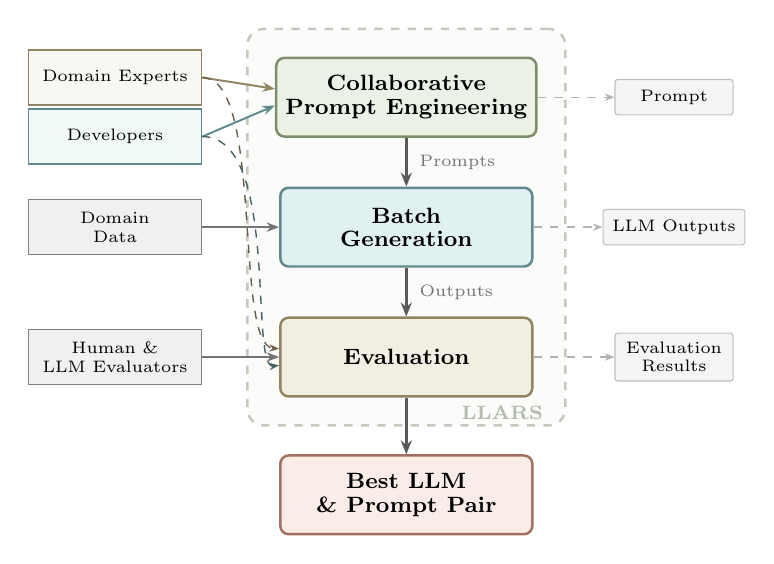
\begin{tikzpicture}[
    module/.style={rectangle, minimum width=3.2cm, minimum height=1.0cm, align=center, font=\footnotesize\bfseries, rounded corners=3pt, line width=0.9pt},
    actor/.style={rectangle, draw=black!50, fill=black!6, minimum width=2.2cm, minimum height=0.7cm, align=center, font=\fontsize{6.5}{8}\selectfont, line width=0.5pt},
    export/.style={rectangle, draw=black!25, fill=black!4, minimum width=1.5cm, minimum height=0.45cm, align=center, font=\fontsize{6}{7.5}\selectfont, rounded corners=1pt},
    outcome/.style={rectangle, draw=clrOutcome!70!black, fill=clrOutcome!20, minimum width=3.2cm, minimum height=1.0cm, align=center, font=\footnotesize\bfseries, rounded corners=3pt, line width=0.9pt},
    arrow/.style={-{Stealth[length=4.5pt]}, line width=0.7pt, black!55},
    pipearrow/.style={-{Stealth[length=5pt, width=4pt]}, line width=1.0pt, black!65},
    dasharrow/.style={-{Stealth[length=3.5pt]}, line width=0.5pt, black!30, dashed},
    lbl/.style={font=\fontsize{6}{7.5}\selectfont, text=black!55},
]

\node[module, draw=clrPrompt!70!black, fill=clrPrompt!25] (pe) at (0, 0) {Collaborative\\[-1pt]Prompt Engineering};
\node[module, draw=clrBatch!70!black, fill=clrBatch!25] (bg) at (0, -1.65) {Batch\\[-1pt]Generation};
\node[module, draw=clrEval!70!black, fill=clrEval!25] (ev) at (0, -3.3) {Evaluation};

% Two actor boxes — same position as original, stacked
\node[rectangle, draw=clrExpert!70!black, fill=clrExpert!12, minimum width=2.2cm, minimum height=0.7cm, align=center, font=\fontsize{6.5}{8}\selectfont, line width=0.5pt] (experts) at (-3.7, 0.25) {Domain Experts};
\node[rectangle, draw=clrDev!70!black, fill=clrDev!12, minimum width=2.2cm, minimum height=0.7cm, align=center, font=\fontsize{6.5}{8}\selectfont, line width=0.5pt] (devs) at (-3.7, -0.5) {Developers};

\node[actor] (data) at (-3.7, -1.65) {Domain\\[-1pt]Data};
\node[actor] (llmeval) at (-3.7, -3.3) {Human \&\\[-1pt]LLM Evaluators};

% Color-coded arrows showing both contribute
\draw[-{Stealth[length=4.5pt]}, line width=0.7pt, clrExpert!70!black] (experts.east) -- ([yshift=3pt]pe.west);
\draw[-{Stealth[length=4.5pt]}, line width=0.7pt, clrDev!70!black] (devs.east) -- ([yshift=-3pt]pe.west);
\draw[arrow] (data.east) -- (bg.west);
\draw[arrow] (llmeval.east) -- (ev.west);

% Color-coded arrows also going to evaluation
\draw[-{Stealth[length=3.5pt]}, line width=0.5pt, clrExpert!50!black, dashed] (experts.east) .. controls (-1.8, 0.25) and (-2.2, -3.15) .. ([yshift=3pt]ev.west);
\draw[-{Stealth[length=3.5pt]}, line width=0.5pt, clrDev!50!black, dashed] (devs.east) .. controls (-1.6, -0.5) and (-2.0, -3.45) .. ([yshift=-3pt]ev.west);

\draw[pipearrow] (pe.south) -- node[lbl, right, xshift=1pt] {Prompts} (bg.north);
\draw[pipearrow] (bg.south) -- node[lbl, right, xshift=1pt] {Outputs} (ev.north);

\node[export] (exp1) at (3.4, 0) {Prompt};
\node[export] (exp2) at (3.4, -1.65) {LLM Outputs};
\node[export] (exp3) at (3.4, -3.3) {Evaluation\\[-1pt]Results};
\draw[dasharrow] (pe.east) -- (exp1);
\draw[dasharrow] (bg.east) -- (exp2);
\draw[dasharrow] (ev.east) -- (exp3);

\node[outcome] (outcome) at (0, -5.05) {Best LLM \\[-1pt]\& Prompt Pair};
\draw[pipearrow] (ev.south) -- (outcome.north);

\begin{scope}[on background layer]
\node[draw=clrPrompt!60!black!40, dashed, rounded corners=6pt, line width=0.9pt, fill=clrPrompt!5, fit=(pe)(bg)(ev), inner xsep=10pt, inner ysep=10pt] (llarsbox) {};
\node[font=\fontsize{7}{9}\selectfont\bfseries, text=clrPrompt!60!black!50, anchor=south east] at ([xshift=-5pt, yshift=-1pt]llarsbox.south east) {LLARS};
\end{scope}

\end{tikzpicture}
\caption{\textbf{J:} Original layout but with color-coded arrows showing both roles participate in Prompt Engineering (solid) and Evaluation (dashed). Shows collaboration without changing the structure.}
\end{figure*}


%% ============================================================
%% VARIANT K: Outside routing, distinct role colors
%% ============================================================

\begin{figure*}[t]
\centering
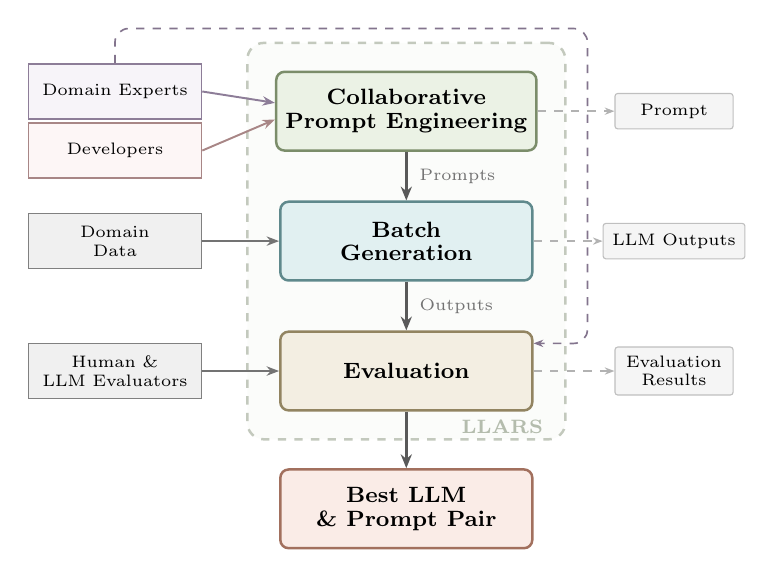
\begin{tikzpicture}[
    module/.style={rectangle, minimum width=3.2cm, minimum height=1.0cm, align=center, font=\footnotesize\bfseries, rounded corners=3pt, line width=0.9pt},
    actor/.style={rectangle, draw=black!50, fill=black!6, minimum width=2.2cm, minimum height=0.7cm, align=center, font=\fontsize{6.5}{8}\selectfont, line width=0.5pt},
    export/.style={rectangle, draw=black!25, fill=black!4, minimum width=1.5cm, minimum height=0.45cm, align=center, font=\fontsize{6}{7.5}\selectfont, rounded corners=1pt},
    outcome/.style={rectangle, draw=clrOutcome!70!black, fill=clrOutcome!20, minimum width=3.2cm, minimum height=1.0cm, align=center, font=\footnotesize\bfseries, rounded corners=3pt, line width=0.9pt},
    arrow/.style={-{Stealth[length=4.5pt]}, line width=0.7pt, black!55},
    pipearrow/.style={-{Stealth[length=5pt, width=4pt]}, line width=1.0pt, black!65},
    dasharrow/.style={-{Stealth[length=3.5pt]}, line width=0.5pt, black!30, dashed},
    lbl/.style={font=\fontsize{6}{7.5}\selectfont, text=black!55},
]

% === Modules ===
\node[module, draw=clrPrompt!70!black, fill=clrPrompt!25] (pe) at (0, 0)
    {Collaborative\\[-1pt]Prompt Engineering};
\node[module, draw=clrBatch!70!black, fill=clrBatch!25] (bg) at (0, -1.65)
    {Batch\\[-1pt]Generation};
\node[module, draw=clrEval!70!black, fill=clrEval!25] (ev) at (0, -3.3)
    {Evaluation};

% === Actor boxes — distinct pastel colors ===
\node[rectangle, draw=clrExpertK!70!black, fill=clrExpertK!15,
      minimum width=2.2cm, minimum height=0.7cm, align=center,
      font=\fontsize{6.5}{8}\selectfont, line width=0.5pt]
      (experts) at (-3.7, 0.25) {Domain Experts};
\node[rectangle, draw=clrDevK!70!black, fill=clrDevK!15,
      minimum width=2.2cm, minimum height=0.7cm, align=center,
      font=\fontsize{6.5}{8}\selectfont, line width=0.5pt]
      (devs) at (-3.7, -0.5) {Developers};

\node[actor] (data) at (-3.7, -1.65) {Domain\\[-1pt]Data};
\node[actor] (llmeval) at (-3.7, -3.3) {Human \&\\[-1pt]LLM Evaluators};

% === Solid colored arrows into Prompt Engineering ===
\draw[-{Stealth[length=4.5pt]}, line width=0.7pt, clrExpertK!70!black]
    (experts.east) -- ([yshift=3pt]pe.west);
\draw[-{Stealth[length=4.5pt]}, line width=0.7pt, clrDevK!70!black]
    (devs.east) -- ([yshift=-3pt]pe.west);
\draw[arrow] (data.east) -- (bg.west);
\draw[arrow] (llmeval.east) -- (ev.west);

% === Outside routing: Domain Experts → Evaluation ===
% Path: up from expert box → right across above LLARS box → down right side → into Evaluation from east
\draw[-{Stealth[length=3.5pt]}, line width=0.6pt, clrExpertK!65!black, dashed, rounded corners=5pt]
    (experts.north) -- (-3.7, 1.05) -- (2.3, 1.05) -- (2.3, -2.95) -- ([yshift=10pt]ev.east);

% === Pipeline arrows ===
\draw[pipearrow] (pe.south) -- node[lbl, right, xshift=1pt] {Prompts} (bg.north);
\draw[pipearrow] (bg.south) -- node[lbl, right, xshift=1pt] {Outputs} (ev.north);

% === Export ===
\node[export] (exp1) at (3.4, 0) {Prompt};
\node[export] (exp2) at (3.4, -1.65) {LLM Outputs};
\node[export] (exp3) at (3.4, -3.3) {Evaluation\\[-1pt]Results};
\draw[dasharrow] (pe.east) -- (exp1);
\draw[dasharrow] (bg.east) -- (exp2);
\draw[dasharrow] (ev.east) -- (exp3);

% === Outcome ===
\node[outcome] (outcome) at (0, -5.05) {Best LLM \\[-1pt]\& Prompt Pair};
\draw[pipearrow] (ev.south) -- (outcome.north);

% === LLARS box ===
\begin{scope}[on background layer]
\node[draw=clrPrompt!60!black!40, dashed, rounded corners=6pt, line width=0.9pt,
      fill=clrPrompt!5, fit=(pe)(bg)(ev),
      inner xsep=10pt, inner ysep=10pt] (llarsbox) {};
\node[font=\fontsize{7}{9}\selectfont\bfseries, text=clrPrompt!60!black!50,
      anchor=south east] at ([xshift=-5pt, yshift=-1pt]llarsbox.south east) {LLARS};
\end{scope}

\end{tikzpicture}
\caption{\textbf{K:} Distinct role colors (lavender = Domain Experts, pink = Developers). Domain Experts participate in both Prompt Engineering (solid) and Evaluation (dashed, routed around the outside of the LLARS box). Cleaner than J's interior routing.}
\end{figure*}


\end{document}
